\documentclass[10pt]{article}
\usepackage[usenames]{color} %used for font color
\usepackage{amssymb} %maths
\usepackage{amsmath} %maths
\usepackage[utf8]{inputenc} %useful to type directly diacritic characters
\usepackage{graphicx,wrapfig}
\usepackage[letterpaper, portrait, margin=1.5in]{geometry}
\usepackage{listings}
\usepackage{color}
\definecolor{dkgreen}{rgb}{0,0.6,0}
\definecolor{gray}{rgb}{0.5,0.5,0.5}
\definecolor{mauve}{rgb}{0.58,0,0.82}
\lstset{frame=tb,
  language=Bash,
  aboveskip=3mm,
  belowskip=3mm,
  showstringspaces=false,
  columns=flexible,
  basicstyle={\small\ttfamily},
  numbers=none,
  numberstyle=\tiny\color{gray},
  keywordstyle=\color{blue},
  commentstyle=\color{dkgreen},
  stringstyle=\color{mauve},
  breaklines=true,
  breakatwhitespace=true,
  tabsize=3
}
\begin{document}
\subsection*{MSDS600 Week 2 Assignment - Nathan Worsham}
Overall my experience in working to accomplish this assignment was relatively pain-free and brisk. I believe however this would not be the experience for all the students in the class which likely is affected by several factors: 
\begin{itemize}
\item I have worked with python before.
\item I have worked with APIs, developer accounts, and developer tokens before.
\item I already have a Twitter account.
\item I am running the latest OS X that already has pip installed and I have used pip before.
\item I am already familiar with capturing output of a command or script.
\end{itemize}
As mentioned I was running my assignment on Mac OS X so it was not necessary to install pip. Next I went ahead and opened terminal and ran the command:
\begin{verbatim}
pip install oauth2 
\end{verbatim}
I received this error: 
\begin{figure}[!h]
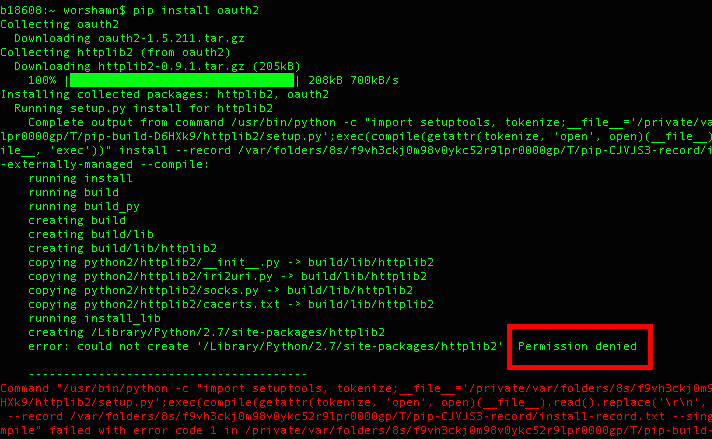
\includegraphics[scale=0.5]{pip_failure2.png}
\centering
\end{figure}



Seeing the error “Permission denied” coupled with the fact that the command it tried to run—setup tools— also “failed” tipped me off that I would need to run this command with root privileges. I have run into this before and really just forgot about it as I was trying to follow the instructions word-for-word. So next I ran the command correctly for my system: 
\begin{verbatim}
sudo pip install oauth2 
\end{verbatim}
The command was successful installing the package this time but still did respond with one issue: \clearpage

\begin{figure}[!h]
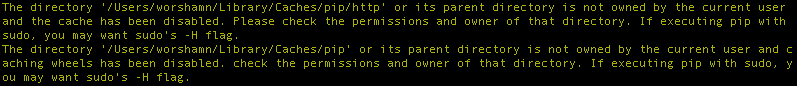
\includegraphics[scale=0.5]{oauth_error.png}
\centering
\end{figure}
\noindent
Looking at the man page for sudo and seeing what the -H flag does, it appears to be about setting the HOME directory of the target user. I am not certain who the target user is in this instance but re-running the command gets the “Requirement already satisfied” message and since I received no further issues I believe the message can be disregarded.  

\begin{wrapfigure}{r}{5cm}
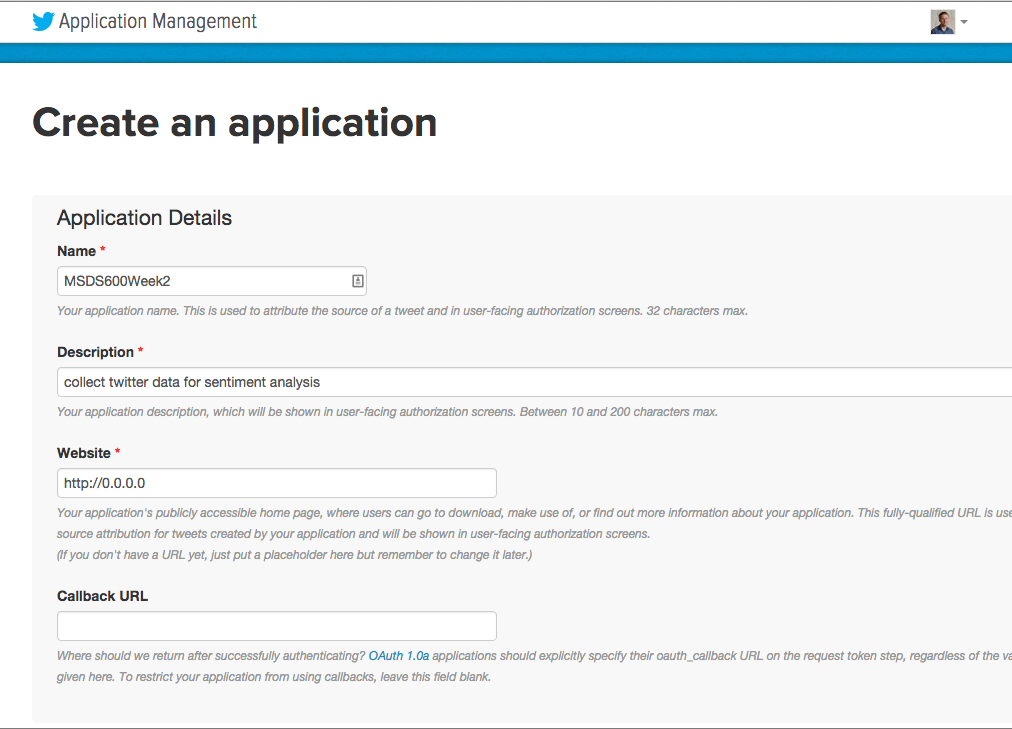
\includegraphics[width=5cm, scale=0.2]{twitter_create.png}
\end{wrapfigure}
I was already logged into Twitter so going to https://dev.twitter.com/apps I was able to immediately click on create app. At this point I was informed that I did not have a mobile phone number associated with my account and would be required to do so in order to continue. I went ahead and did as asked by adding my mobile number (which I imagine is data that Twitter is more than happy to collect, I have not read their terms of service, but it represents another NULL value conquered and more data ready to sell/exchange/barter to a waiting line of third parties). \\*
\begin{figure}[!h]

\includegraphics[scale=0.3]{twitter_error.png}
\centering
\end{figure}\\
Now I was able to create the app and fill out the form. For the dummy website I used http://0.0.0.0--this is an address I am accustomed to using in test API accounts. As wikipedia (n.d.) puts it "the address 0.0.0.0 is a non-routable meta-address used to designate an invalid, unknown or non-applicable target”.  
\begin{figure}[!h]

\includegraphics[scale=0.4]{twitter_created2.png}
\centering
\end{figure}\\*
Next I realized that the API key and token would need to be generated, so after generating these I was ready to copy and paste the values into the python script:
\begin{figure}[!h]
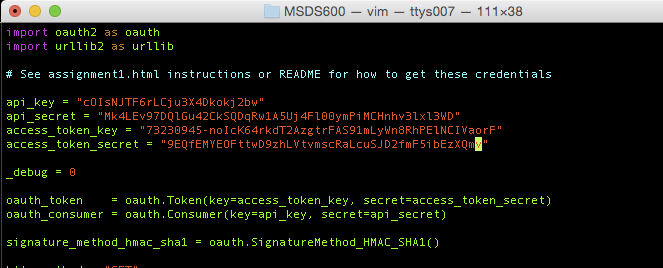
\includegraphics[scale=0.5]{twitter_apikeys.png}
\centering
\end{figure}

Finally I ran the command \verb|python twitterstream.py > output.txt| for a few seconds and then checked the contents with \verb|tail| to be sure I was getting what was expected which turned out to be good:
\begin{figure}[!h]
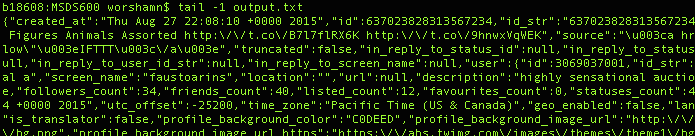
\includegraphics[scale=0.5]{tail.png}
\centering
\end{figure}\\*
\noindent 
I then ran the command for the 3 minutes as required. After the time was up I used \verb|cat| and \verb|wc -l| to see how many lines I had collected which was 9619:
\begin{figure}[!h]
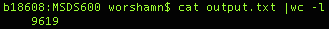
\includegraphics[scale=1]{cat_output.png}
\end{figure}
\subsection*{Reference}
Wikipedia (n.d.) Retrieved from https://en.wikipedia.org/wiki/0.0.0.0
\end{document}